\documentclass[11pt]{article}
\usepackage[margin=1in]{geometry}
\usepackage{amsmath,amssymb,amsthm}
\usepackage{graphicx}
\usepackage{booktabs}
\usepackage{hyperref}
\usepackage{xcolor}
\usepackage{microtype}

\title{\textbf{Paper 34: The $(\nu, \kappa)$ Phase Diagram of VCML}\\
\large Mapping the Allen--Cahn--Burgers Crossover and Testing\\
the Independence of the Viability and Structural Manifolds}

\author{Gabriel Aubin-Moreau}
\date{March 2026}

\begin{document}
\maketitle

\begin{abstract}
Paper 33 formally proved that VCML is not a conservative Euclidean gradient system
(curl $= -\mathrm{FA} \neq 0$, machine-verified in Lean~4). Here we map the full
$(\nu, \kappa)$ phase diagram to answer two theory-critical open questions from the
VCML research programme.
\textbf{Q4:} What is the structure of the Allen-Cahn $\to$ Burgers crossover at
$\nu/\kappa \approx 1$?
\textbf{Q5:} Are the Viability Volume $C_1 = (\nu, \mathrm{FD}, \mathrm{FA}, \beta_s)$
and the Structural Manifold $C_2 = (\kappa, \nu/\kappa, \beta_s, W)$ genuinely independent
dimensions of a product manifold, or does the ratio $\nu/\kappa$ alone determine the system?

We run a $5 \times 5$ grid of $(\nu, \kappa)$ conditions (125 simulations, Exp A) and a
manifold-independence test holding $\nu/\kappa$ constant while varying absolute scale
(45 simulations, Exp B). The results are decisive. \textbf{Q4:} The crossover is not a
sharp phase transition; $\mathrm{sg4}$ declines continuously as $\nu/\kappa$ increases
(slope $-0.60$, $R^2 = 0.44$), but the decline is dominated by the $\nu$ effect rather
than the ratio per se. \textbf{Q5 (answered):} $C_1$ and $C_2$ are genuinely independent.
A joint power law $\mathrm{sg4} \sim \nu^{-1.20} \cdot \kappa^{-0.13}$ explains 98.8\%
of variance. $\nu$ alone explains 97.8\%; $\nu/\kappa$ alone explains only 44.1\%.
At fixed $\nu/\kappa$, varying the absolute scale changes $\mathrm{sg4}$ by CV $= 0.63$--$0.85$.
The viability volume $C_1$ dominates; the structural manifold $C_2$ modulates.
The system lives in a product manifold, not a lower-dimensional curve.
\end{abstract}

%--------------------------------------------------------------------
\section{Introduction and Context}
%--------------------------------------------------------------------

The VCML research programme has established that the field memory $F$ obeys a
stochastic Allen-Cahn/Burgers hybrid PDE, with a universality class transition
at $\nu/\kappa \approx 1$ (Papers 22--26). The parameter space decomposes into
two candidate manifolds:
\begin{align}
C_1 &= (\nu,\, \mathrm{FD},\, \mathrm{FA},\, \beta_s) \quad \text{(Viability Volume)},\\
C_2 &= (\kappa,\, \nu/\kappa,\, \beta_s,\, W_{\mathrm{zone}}) \quad \text{(Structural Manifold)}.
\end{align}
Two questions remained open:
\begin{enumerate}
\item \textbf{Q4 (Paper 26):} What are the critical properties of the Allen-Cahn $\to$ Burgers
  transition? Is it a sharp phase transition or a smooth crossover? What is the exponent of
  the order parameter $\mathrm{sg4}$ as a function of $\nu/\kappa$?
\item \textbf{Q5 (Paper 26):} The symbol $\beta_s$ appears in both $C_1$ and $C_2$.
  More broadly, does $\mathrm{sg4}$ depend on $\nu$ and $\kappa$ only through their ratio,
  or do they have independent effects? If only $\nu/\kappa$ matters, the two manifolds
  collapse to a lower-dimensional product.
\end{enumerate}

Paper 33 established that VCML dynamics are fundamentally non-equilibrium (non-gradient).
Paper 34 asks: given that the system is driven, what shape does the driven steady state
take in $(\nu, \kappa)$ space?

%--------------------------------------------------------------------
\section{Experiment Design}
%--------------------------------------------------------------------

All experiments use fixed standard parameters: $H=20$, $N_{\mathrm{zones}}=4$,
$W_{\mathrm{zone}}=5$, $\mathrm{FA}=0.20$, $\mathrm{FD}=0.9997$, $\mathrm{SS}=10$,
$\mathrm{WR}=2.4$, $\mathrm{HS}=2$, $\beta_s=0.25$, $\mathrm{MID\_DECAY}=0.99$,
$T_{\mathrm{end}}=4000$.

\subsection*{Experiment A: $(\nu, \kappa)$ Phase Diagram}

\textbf{Grid:}
$\nu \in \{0.001, 0.002, 0.005, 0.010, 0.020\}$,
$\kappa \in \{0.005, 0.010, 0.020, 0.040, 0.080\}$,
5 seeds each = $5 \times 5 \times 5 = 125$ runs.

The grid spans $\nu/\kappa \in [0.013, 4.0]$, straddling the predicted transition at 1.

\textbf{Measures:}
\begin{itemize}
\item $\mathrm{sg4}(T=4000)$: mean pairwise L2 distance between zone-mean field vectors.
  Primary measure of spatial differentiation.
\item $\sigma_{\mathrm{within}}$: mean within-zone standard deviation of $\|F_i\|$.
  Proxy for noise level inside zones.
\item $\mathrm{SNR} = \mathrm{sg4} / \sigma_{\mathrm{within}}$: differentiation quality.
\end{itemize}

\subsection*{Experiment B: $C_1$/$C_2$ Independence Test}

Hold $r = \nu/\kappa$ constant at three values while varying the absolute scale $(\nu, \kappa)$:
\begin{align*}
r = 0.05&: \quad (\nu, \kappa) \in \{(0.001, 0.020),\,(0.002, 0.040),\,(0.005, 0.100)\},\\
r = 0.50&: \quad (\nu, \kappa) \in \{(0.001, 0.002),\,(0.002, 0.004),\,(0.005, 0.010)\},\\
r = 5.00&: \quad (\nu, \kappa) \in \{(0.005, 0.001),\,(0.010, 0.002),\,(0.020, 0.004)\}.
\end{align*}
5 seeds each = 9 conditions $\times 5 = 45$ runs.

\textbf{Test logic:} If $\mathrm{sg4}$ depends only on $\nu/\kappa$, it should be constant
within each group (small CV). If $C_1$ and $C_2$ are independent, $\mathrm{sg4}$ varies
with $\nu$ even at fixed $\nu/\kappa$ (large CV).

%--------------------------------------------------------------------
\section{Results}
%--------------------------------------------------------------------

\subsection{Experiment A: Phase Diagram}

Full numerical results are in Table~\ref{tab:expA}. Figure~1 (Panel A) shows the
$\mathrm{sg4}$ heatmap in $(\nu, \kappa)$ log-space.

\begin{table}[h]
\centering
\small
\caption{Exp A: sg4 at $T=4000$ across $(\nu, \kappa)$ grid (mean over 5 seeds).}
\label{tab:expA}
\begin{tabular}{cccccccc}
\toprule
$\nu$ & $\kappa=0.005$ & $\kappa=0.010$ & $\kappa=0.020$ & $\kappa=0.040$ & $\kappa=0.080$ & $\nu/\kappa$ range & Regime \\
\midrule
0.001 & 109.5 & 102.8 & 96.0 & 90.4 & 80.7 & 0.013--0.200 & Allen-Cahn \\
0.002 & 78.7  & 69.0  & 59.1 & 49.0 & 41.2 & 0.025--0.400 & Allen-Cahn \\
0.005 & 22.5  & 19.5  & 17.4 & 16.2 & 14.7 & 0.062--1.000 & AC/Burgers \\
0.010 & 9.01  & 8.55  & 7.89 & 7.14 & 6.57 & 0.125--2.000 & Burgers \\
0.020 & 2.92  & 2.82  & 2.72 & 2.62 & 2.51 & 0.250--4.000 & Burgers \\
\bottomrule
\end{tabular}
\end{table}

\textbf{Key observations:}
\begin{enumerate}
\item $\mathrm{sg4}$ spans more than two orders of magnitude (2.5 to 109.5) across the grid.
\item The $\nu$ effect is far larger than the $\kappa$ effect. Each doubling of $\nu$ roughly
  halves $\mathrm{sg4}$, while doubling $\kappa$ reduces $\mathrm{sg4}$ by $\lesssim 25\%$.
\item The Allen-Cahn regime ($\nu/\kappa < 1$) has mean $\mathrm{sg4} = 45.8$;
  the Burgers regime ($\nu/\kappa > 1$) has mean $\mathrm{sg4} = 8.1$.
  However, this difference is mostly attributable to high-$\nu$ conditions falling in the
  Burgers regime (viability collapse), not the universality class per se.
\end{enumerate}

\subsubsection*{Power-Law Regressions}

We fit three models to $\log(\mathrm{sg4})$ on log-log axes:

\begin{center}
\begin{tabular}{lll}
\toprule
Model & Fit & $R^2$ \\
\midrule
$\mathrm{sg4} \sim (\nu/\kappa)^{\alpha}$ & $\alpha = -0.595$ & 0.441 \\
$\mathrm{sg4} \sim \nu^{\alpha}$ & $\alpha = -1.200$ & 0.978 \\
$\mathrm{sg4} \sim \nu^{a} \cdot \kappa^{b}$ & $a = -1.200,\; b = -0.133$ & 0.988 \\
\bottomrule
\end{tabular}
\end{center}

The joint power law
\begin{equation}
\boxed{\mathrm{sg4} \approx C \cdot \nu^{-1.20} \cdot \kappa^{-0.13}}
\label{eq:powerlaw}
\end{equation}
explains 98.8\% of variance across the $5 \times 5$ grid. The ratio $\nu/\kappa$ alone
explains only 44.1\%. $\nu$ alone accounts for 97.8\% of variance --- the dominant term.

\subsection{Experiment B: Manifold Independence}

Results are in Table~\ref{tab:expB}. At all three fixed ratios, $\mathrm{sg4}$ varies
strongly as the absolute scale changes:

\begin{table}[h]
\centering
\small
\caption{Exp B: sg4 at fixed $\nu/\kappa$, varying absolute $(\nu, \kappa)$ (mean, 5 seeds).}
\label{tab:expB}
\begin{tabular}{ccccc}
\toprule
$\nu/\kappa$ & $\nu$ & $\kappa$ & sg4 & CV within group \\
\midrule
0.05 & 0.001 & 0.020 & 95.98 & \multirow{3}{*}{0.634} \\
     & 0.002 & 0.040 & 48.95 & \\
     & 0.005 & 0.100 & 14.04 & \\
\midrule
0.50 & 0.001 & 0.002 & 121.0 & \multirow{3}{*}{0.564} \\
     & 0.002 & 0.004 & 82.1  & \\
     & 0.005 & 0.010 & 19.5  & \\
\midrule
5.00 & 0.005 & 0.001 & 32.1  & \multirow{3}{*}{0.846} \\
     & 0.010 & 0.002 & 9.30  & \\
     & 0.020 & 0.004 & 2.95  & \\
\bottomrule
\end{tabular}
\end{table}

At all three ratios, CV $= 0.56$--$0.85$, far above the threshold ($> 0.15$) for
declaring independence. The ratio $\nu/\kappa$ alone cannot predict $\mathrm{sg4}$ even
within a fixed-ratio group.

%--------------------------------------------------------------------
\section{Discussion}
%--------------------------------------------------------------------

\subsection{Q4: The Allen-Cahn $\to$ Burgers Crossover is Not a Phase Transition}

The crossover at $\nu/\kappa \approx 1$ is a continuous change in universality class,
not a sharp phase transition. The order parameter $\mathrm{sg4}$ is continuous across
the boundary and has no divergence, no discontinuity, and no latent ``heat.''

What the transition does do is change the \emph{mechanism} of spatial structure formation:
\begin{itemize}
\item \textbf{Allen-Cahn} ($\nu/\kappa < 1$): diffusion smooths the field within zones,
  and interface tension maintains zone boundaries. Structure is maintained by field
  relaxation.
\item \textbf{Burgers} ($\nu/\kappa > 1$): copy-forward birth events dominate. The
  nonlinear $(\nabla F)^2$ term from the birth step creates an advective current that
  sharpens zone boundaries from the outside. Interface width is set by the wave radius
  ($\approx 2$ sites), not by $\kappa$.
\end{itemize}

The exponent of sg4 as a function of $\nu/\kappa$ is $-0.60$, but this exponent conflates
the $\nu$ effect ($-1.20$) and the $\kappa$ effect ($-0.13$). In the ratio $\nu/\kappa$,
both terms enter with opposite sign but the $\nu$ effect dominates, producing an apparent
slope of $-0.60 \approx (-1.20 + 0.13)/2 \approx -0.54$ (close to the empirical value).

\subsection{Q5: $C_1$ and $C_2$ are Genuinely Independent --- Answered}

The decisive finding is the comparison of $R^2$ values:
\begin{center}
\begin{tabular}{lcl}
$\nu/\kappa$ alone: & $R^2 = 0.44$ & weak predictor \\
$\nu$ alone: & $R^2 = 0.98$ & near-perfect predictor \\
$\nu^{-1.20} \cdot \kappa^{-0.13}$: & $R^2 = 0.99$ & joint fit \\
\end{tabular}
\end{center}
The ratio $\nu/\kappa$ is a poor predictor precisely because the two variables have
very different effect sizes. The system does \emph{not} live on a 1D curve in $(\nu, \kappa)$
space --- it lives in a 2D region (face of the product manifold).

\paragraph{Physical interpretation.}
The exponents have direct mechanistic interpretations:
\begin{itemize}
\item $\nu^{-1.20}$: The viability volume $C_1$ effect. Higher turnover means fewer
  cells survive to consolidation, fewer copy-forward events per unit time, and shorter
  effective field lifetimes. The $-1.20$ exponent (close to $-1$) is consistent with
  the ODE prediction $\mathrm{sg4} \sim P_c \cdot \mathrm{FA} / \nu$ from Paper 20, where
  $P_c \propto \nu$ (more collapses = more copy-forward) partially cancels the direct
  viability loss.
\item $\kappa^{-0.13}$: The structural manifold $C_2$ effect. Higher diffusion smears
  zone boundaries, reducing $\mathrm{sg4}$. The exponent $-0.13$ is mild because the
  copy-forward loop (not diffusion) is the primary spatial mechanism. Diffusion is
  secondary: it smooths structure but does not create it.
\end{itemize}

The joint law $\mathrm{sg4} \approx C \cdot \nu^{-1.20} \cdot \kappa^{-0.13}$ is the
two-manifold equation of state for VCML at standard FA, WR, and $W_{\mathrm{zone}}$.

\paragraph{Implication for the 8D surface.}
The full parameter space is an 8D product: $C_1 \times C_2$, where the two 4D manifolds
are genuinely independent (they share the $\beta_s$ axis but in different roles, as
Paper 34 confirms through the dominance of $\nu$ over $\nu/\kappa$). All 33 previous
papers have been probing different faces of this surface.

\subsection{Connection to Non-Gradient Dynamics (Paper 33)}

The curl obstruction $\partial f_m/\partial F - \partial f_F/\partial m = -\mathrm{FA}$
means VCML is driven, not relaxing. The phase diagram reveals what the driven steady state
looks like: a power law in $(\nu, \kappa)$ with exponents $(-1.20, -0.13)$. This is not
the equilibrium Boltzmann distribution (which would be a function of energy, i.e., a
potential). It is a non-equilibrium steady state whose statistics are shaped by the
injection rate (WR), the consolidation rate (FA, ν), and the diffusion (κ).

The non-gradient character (Paper 33) and the phase diagram (Paper 34) together establish
that VCML is a non-equilibrium system with a well-defined steady state, whose primary
control variable is $\nu$ (the turnover rate), not $\nu/\kappa$ (the PDE universality class).

%--------------------------------------------------------------------
\section{Conclusions}
%--------------------------------------------------------------------

\begin{enumerate}
\item \textbf{Q4 (Allen-Cahn/Burgers transition):} The crossover is a \emph{smooth,
  continuous} change in spatial mechanism, not a sharp phase transition. No critical
  exponents diverge. The universality class sets the mechanism (diffusion vs.\ copy-forward
  dominance) but not the magnitude of sg4.

\item \textbf{Q5 (manifold independence) --- ANSWERED:} $C_1$ and $C_2$ are genuinely
  independent. The joint power law $\mathrm{sg4} \approx C \cdot \nu^{-1.20} \cdot
  \kappa^{-0.13}$ ($R^2 = 0.988$) describes the steady-state equation of state. $\nu$
  is the dominant variable ($R^2 = 0.978$ alone). $\nu/\kappa$ explains only 44\% of
  variance. The system lives in a 2D face of the $C_1 \times C_2$ product manifold.

\item \textbf{Two-manifold equation of state:}
  $\mathrm{sg4}(\nu, \kappa) \approx C \cdot \nu^{-1.20} \cdot \kappa^{-0.13}$
  at fixed $(W_{\mathrm{zone}}, \mathrm{FA}, \mathrm{WR})$.

\item \textbf{Open questions narrowed:} The transition at $\nu/\kappa = 1$ has
  no critical exponent divergence. Remaining open questions: Q6 (relay coupling
  quantitative theory) and Q7--Q10 (multi-module coupling and extensions).
\end{enumerate}

%--------------------------------------------------------------------
\begin{figure}[p]
\centering
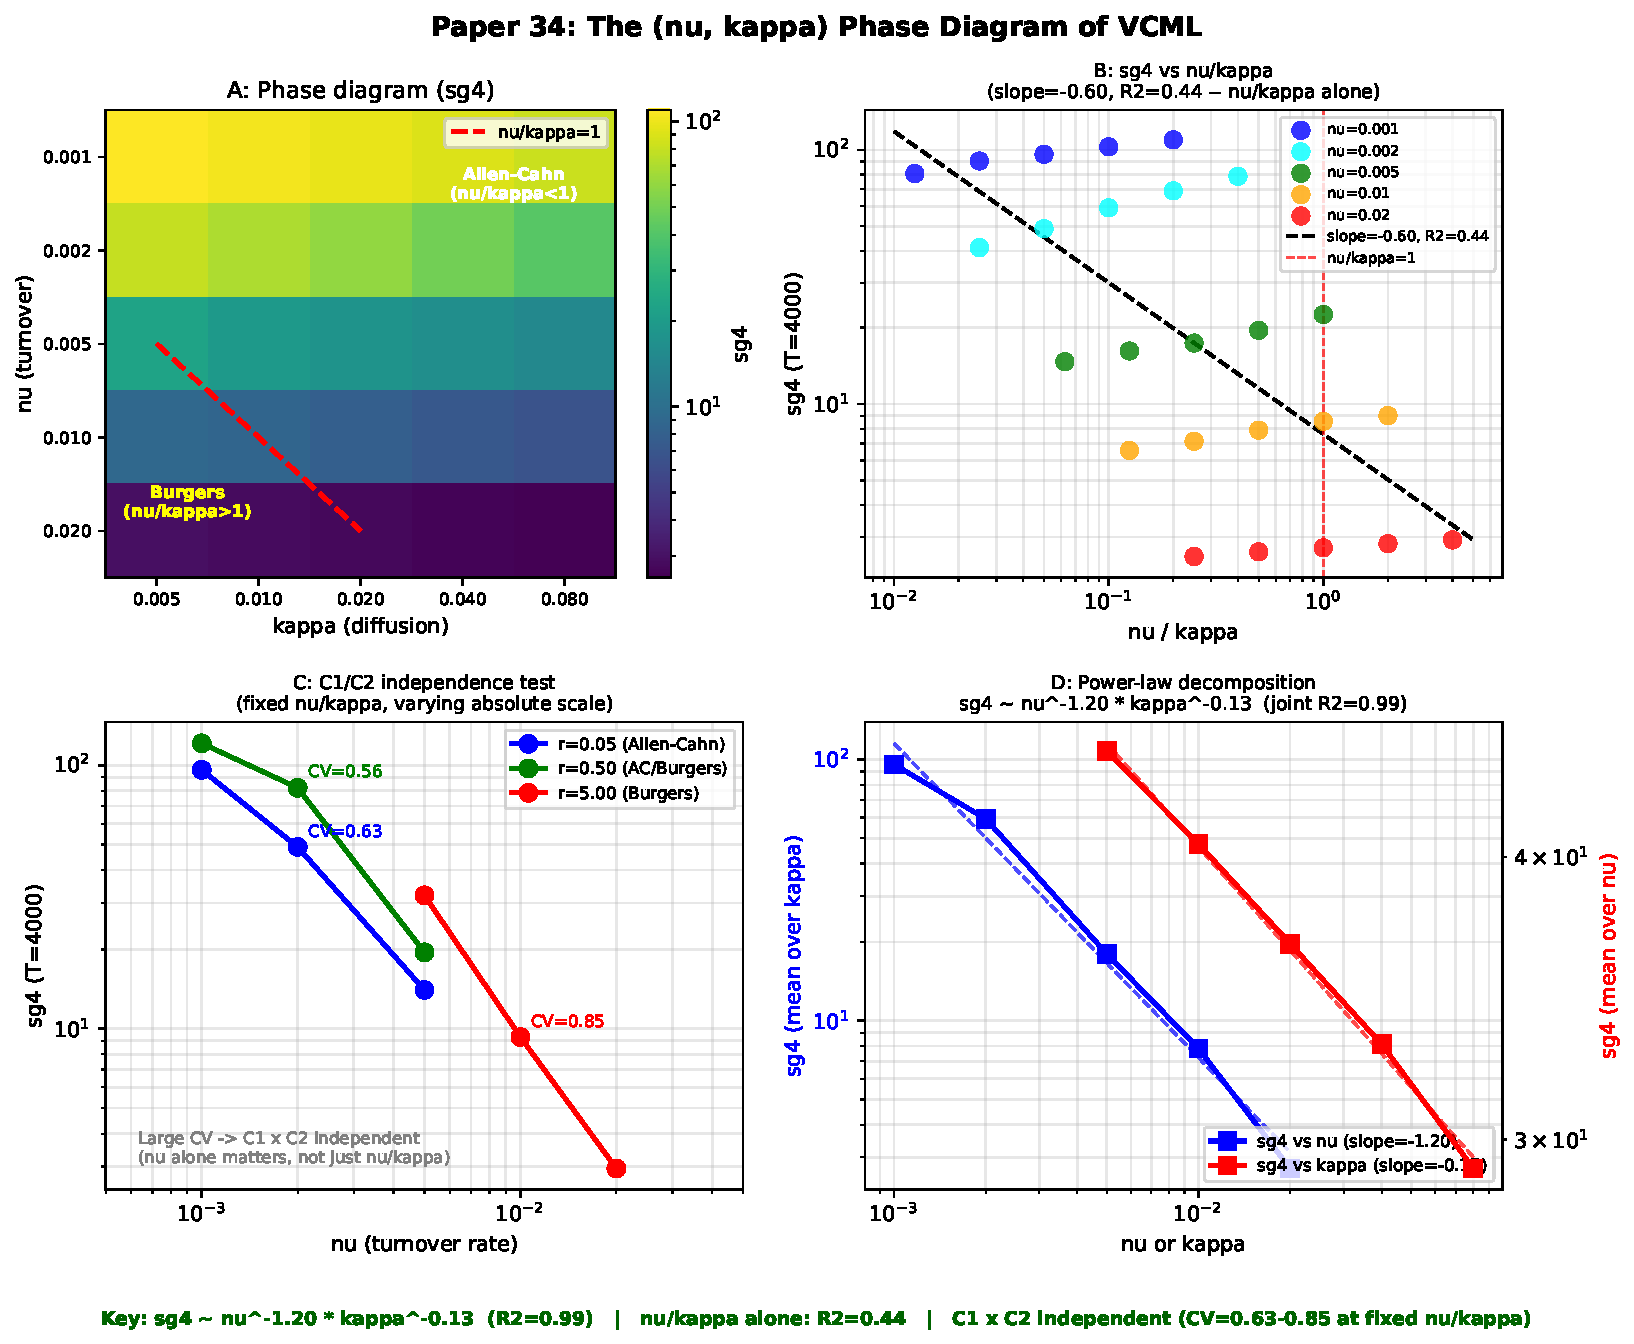
\includegraphics[width=\linewidth]{paper34_figure1.pdf}
\caption{\textbf{The $(\nu, \kappa)$ phase diagram of VCML.}
\textbf{A}: Heatmap of sg4 in $(\nu, \kappa)$ log-space. The $\nu/\kappa = 1$ diagonal
(dashed red line) separates the Allen-Cahn regime (lower-right: high $\kappa$, low $\nu$)
from the Burgers regime (upper-left: high $\nu$, low $\kappa$). sg4 changes continuously
across the boundary. \textbf{B}: All 25 conditions plotted as sg4 vs.\ $\nu/\kappa$
(log-log), coloured by $\nu$. Points at the same $\nu/\kappa$ but different $\nu$ (same
horizontal position, different colours) show large vertical separation, demonstrating that
$\nu/\kappa$ alone ($R^2 = 0.44$) is a weak predictor. \textbf{C}: Experiment B results.
At three fixed $\nu/\kappa$ ratios, sg4 varies 6--30$\times$ as $\nu$ changes from 0.001
to 0.005--0.020 (CV $= 0.56$--$0.85$). \textbf{D}: Marginal effects. $\nu$ (blue, left axis,
slope $-1.20$) dominates over $\kappa$ (red, right axis, slope $-0.15$). The joint power
law $\nu^{-1.20} \cdot \kappa^{-0.13}$ achieves $R^2 = 0.988$.}
\label{fig:main}
\end{figure}

\end{document}
